\newcommand{\chtwopin}{{\constant 13}\xspace}

By changing just one line of code, you can control the speed at which the LED on your Arduino blinks.

\GOALS
This chapter just takes a small step from Chapter~\ref{ch1}.
\begin{enumerate}
	\item Build our first circuit.
	\item See how digital voltages are either \HIGH or \LOW.
	\item Learn about the \blink procedure in \plumbing.
	\item Learn how to control the behavior of a procedure by changing its parameters.	

\end{enumerate}


\section{Building the Circuit}
%You now have enough \plumbing code to add an LED to your Arduino, and control it {\em instead} of the LED on the board!
We could just blink the built-in LED, but we need to know how to connect multiple LEDs to the Arduino if we're going to work through Chapter~\ref{ch3}:~\nameref{ch3}, where we'll learn to blink both the built-in and external LEDs at the same time.

% FIXME Replace me with a hand-drawn picture?
%\begin{figure}[ht]
%  \begin{center}
%    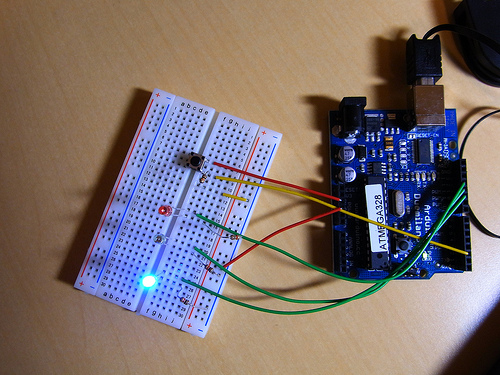
\includegraphics[width=\linewidth]{images/one-led}
%    \caption{Connect up one LED to your Arduino.}
%    \label{circuit:one-led}
%  \end{center}
%\end{figure}

Your Arduino will live at the center of a number of increasingly complex circuits. We call them {\em circuits} because they are a loop that makes an electrical connection from a voltage source (in this case, pin \chtwopin), through one or more electronic components back to ``ground'' (typically labeled {\code GND}). Our goal is a circuit that looks like Figure~\vref{diagram:ch2-one-led-circuit}.

\begin{figure}[ht]
  \begin{center}
    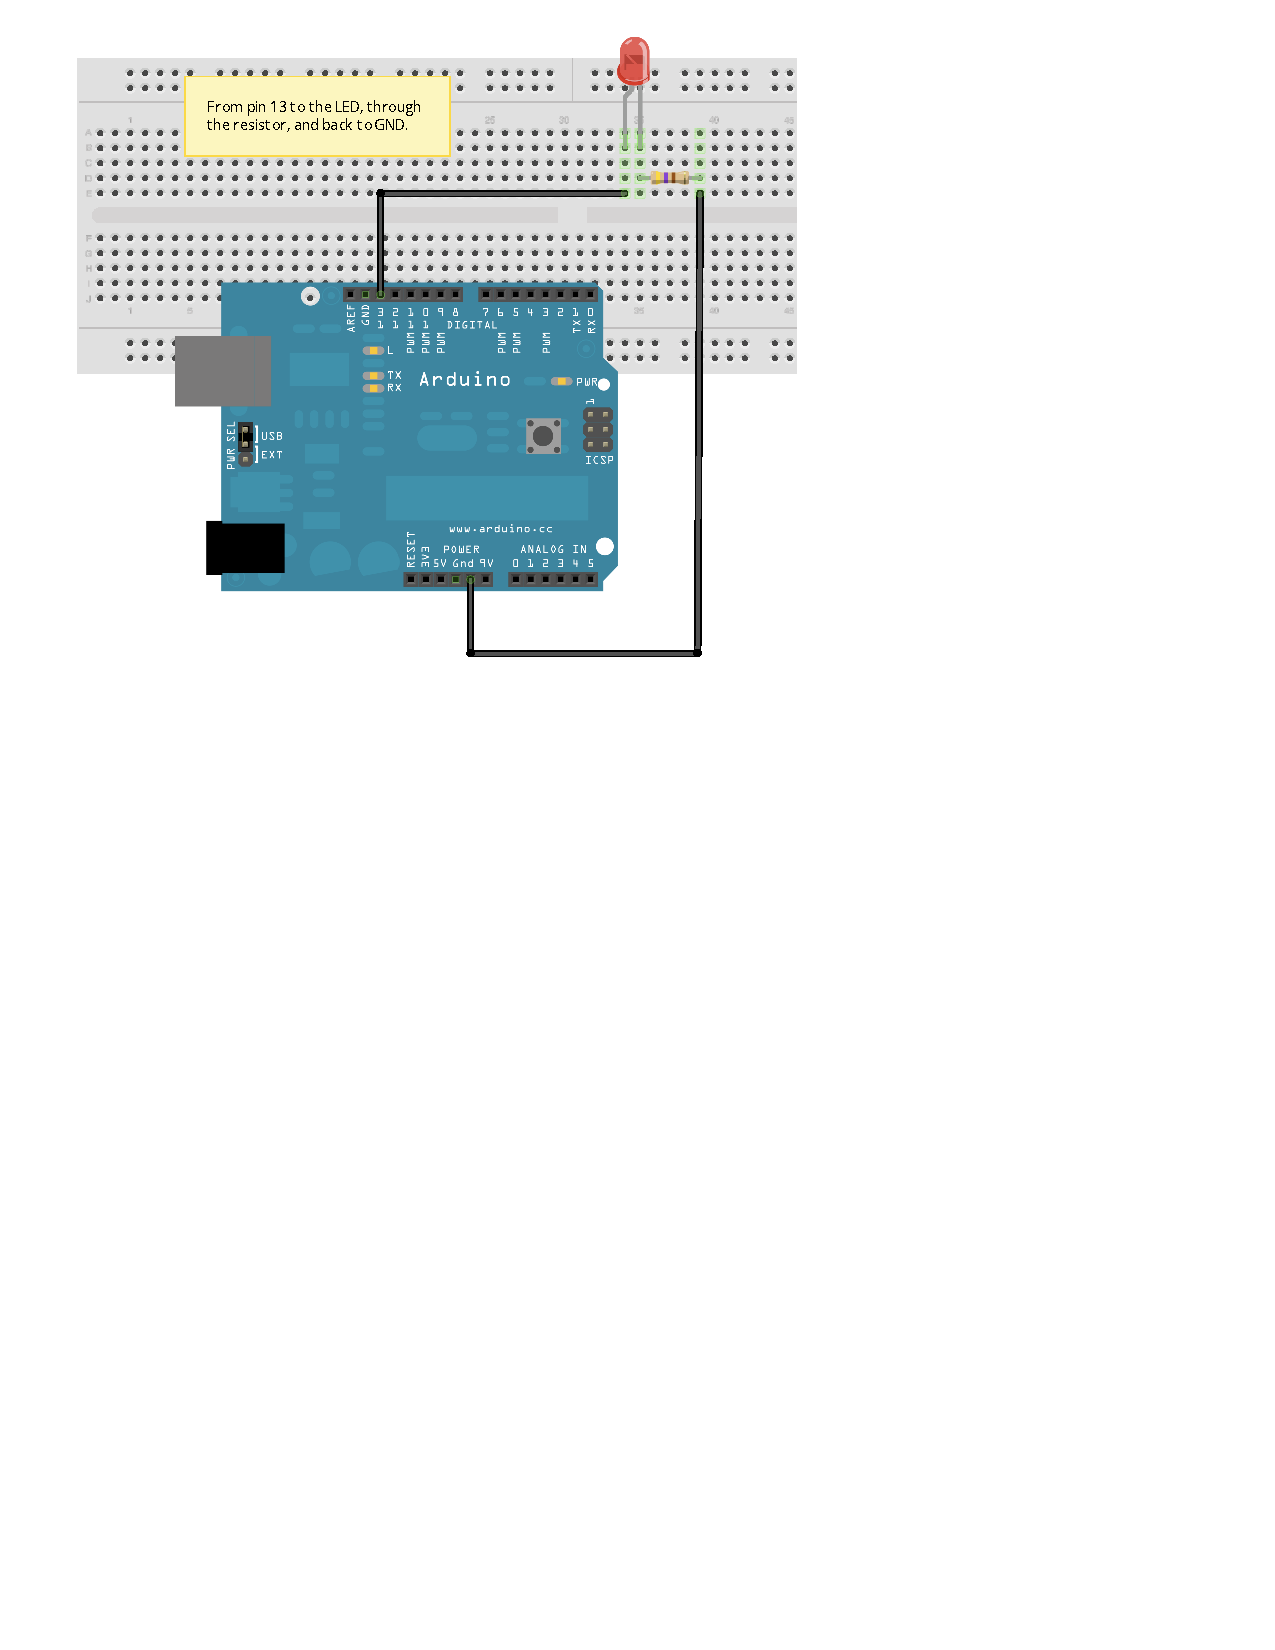
\includegraphics[width=0.95\linewidth]{images/ch2-one-led-circuit}
    \caption{Our target circuit.}
    \label{diagram:ch2-one-led-circuit}
  \end{center}
\end{figure}

\newpage

To connect up another LED, you're going to need:

\begin{enumerate}
	\item A breadboard
	\item An LED
	\item A resistor (with a value between 470\ohm and 1000\ohm)
	\item Some jumper wires
	\item Your Arduino
\end{enumerate}

\begin{floatingfigure}[r]{0.5\linewidth}
	  \begin{center}
    	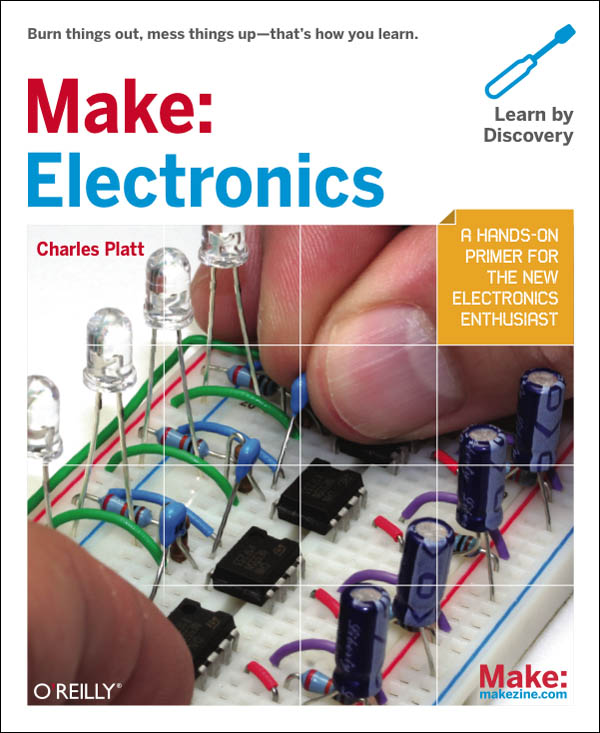
\includegraphics[width=0.4\linewidth]{images/make-electronics-cover}
			\captionsetup{labelformat=empty,justification=centering,font=footnotesize}
   		\caption{A good resource.}
    	%\label{screenshot:compile-successful}
  \end{center}
\end{floatingfigure}

We'll build the circuit up one step at a time. What we won't be doing is teaching you electronics---for that, we recommend you pick up a copy of {\em Make: Electronics}\webnote{http://oreilly.com/catalog/9780596153755/}{\em Make: Electronics}, or for a more in-depth treatment, perhaps a used copy of {\em The Art of Electronics}\webnote{http://frank.harvard.edu/aoe/}{{\em The Art of Electronics}} by Horowitz and Hill. Because this is our first circuit, we'll take a bit more time, but in future chapters, we'll be assuming that you have a resource like {\em Make: Electronics} available to you. This is more a book about programming with \plumbing than a book about the fundamentals of electronic circuit design.

\newpage

\subsection{The Breadboard}
The breadboard provides a foundation for building and testing small circuits. Breadboards come in many shapes and sizes; if you have a small Arduino kit, you might have a breadboard like that pictured in Figure~\vref{diagram:ch2-little-red-breadboard-connections}. Note that things in a column (on one side of the gutter) are connected, but things on opposite sides of the gutter are not. 

\begin{figure}[ht]
  \begin{center}
    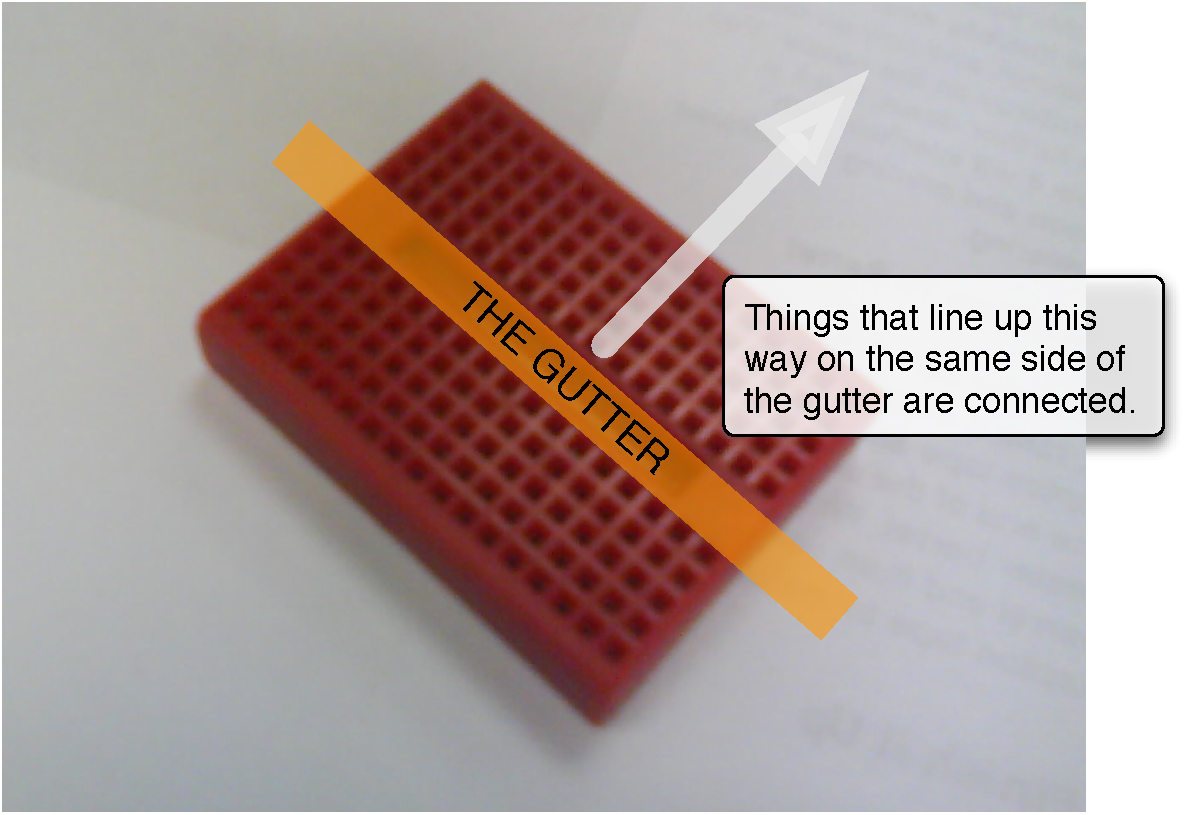
\includegraphics[width=0.8\linewidth]{images/ch2-little-red-breadboard-connections}
    \caption{How a breadboard works.}
    \label{diagram:ch2-little-red-breadboard-connections}
  \end{center}
\end{figure}

\subsection{The Arduino}
With the Arduino turned off (unplugged from the USB port), take a wire and connect it from pin \chtwopin to one of the columns in the breadboard. Perhaps start with the left-most column, and we'll build our circuit from left-to-right. (See ~\vref{diagram:ch2-one-led-circuit} if you get confused---it's rather accurate.) 

\subsection{The Resistor}
\begin{wrapfigure}{r}{0.4\linewidth}
	  \begin{center}
    	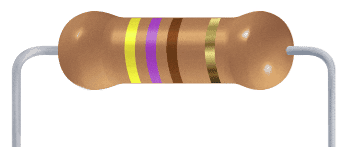
\includegraphics[width=0.9\linewidth]{images/20100109-470-ohm-resistor}
			\captionsetup{labelformat=empty,justification=centering}%,font=footnotesize}
   		\caption{A 470\ohm resistor.}
    	%\label{screenshot:compile-successful}
  \end{center}
\end{wrapfigure}

If you plug your LED directly into an electronic device---even one as small as the Arduino---you might burn it out. If you manage this, it will probably flash brightly once and never light again. Therefore, we need a resistor to help limit the flow of current through our circuit so the LED doesn't get fried. If you need a rule of thumb (which is not always correct!), a 1K\ohm resistor is typically more than enough to protect your LED.\footnote{If you want something better than a guideline, look up Ohm's Law on the Wikipedia: \url{http://en.wikipedia.org/wiki/Ohms\_law}.}

Resistors are the little barrel-shaped things with different colored stripes on them. Those stripes tell you what resistance value they have.\webnote{http://en.wikipedia.org/wiki/Electronic_color_code}{the color codes on resistors} Plug one end of the 470\ohm resistor (\resistor{Yellow}{Purple}{Brown}, Yellow Purple Brown Gold) into the same column of the breadboard as the wire you connected from the Arduino, and the other into an unused column further to the right. 



\subsection{The LED}
LEDs are a kind of diode. A diode is a device that only allows electric current to flow in one direction. Therefore, if you connect an LED up ``backwards,'' nothing will happen. (This is true up to a point---enough current will destroy an LED even in a backwards configuration.) 

\begin{figure}[ht]
  \begin{center}
    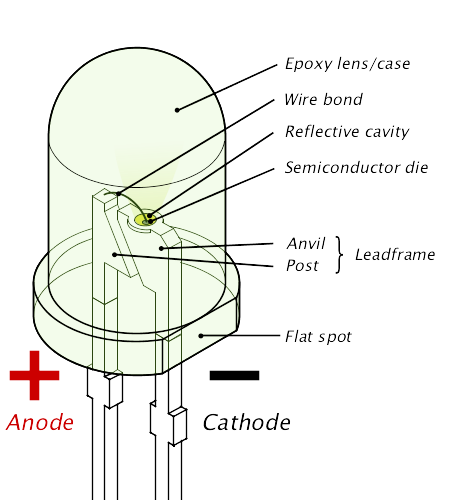
\includegraphics[width=0.5\linewidth]{images/ch2-led-internals}
    \caption{The internals of an LED.}
    \label{diagram:ch2-led-internals}
  \end{center}
\end{figure}

Some people say ``the long leg of the LED is the negative leg.'' This is true, but if your LED gets mangled, it becomes difficult to tell which leg is which. Instead, look at Figure~\vref{diagram:led-internals}, and find the ``anvil.'' The anvil is the larger of the two bits inside the LED, and it is {\em always} the negative side of the LED, meaning the ``post'' is {\em always} the positive side.\footnote{See \url{http://en.wikipedia.org/wiki/Led} for more information.}

Plug your LED into the breadboard so that the positive side is in the same column as your jumper wire from \chtwopin, and the negative side is in a column with one end	 of your resistor.

\subsection{Completing the circuit}

%\begin{figure}[ht]
\begin{wrapfigure}{r}{0.45\linewidth}
  \begin{center}
    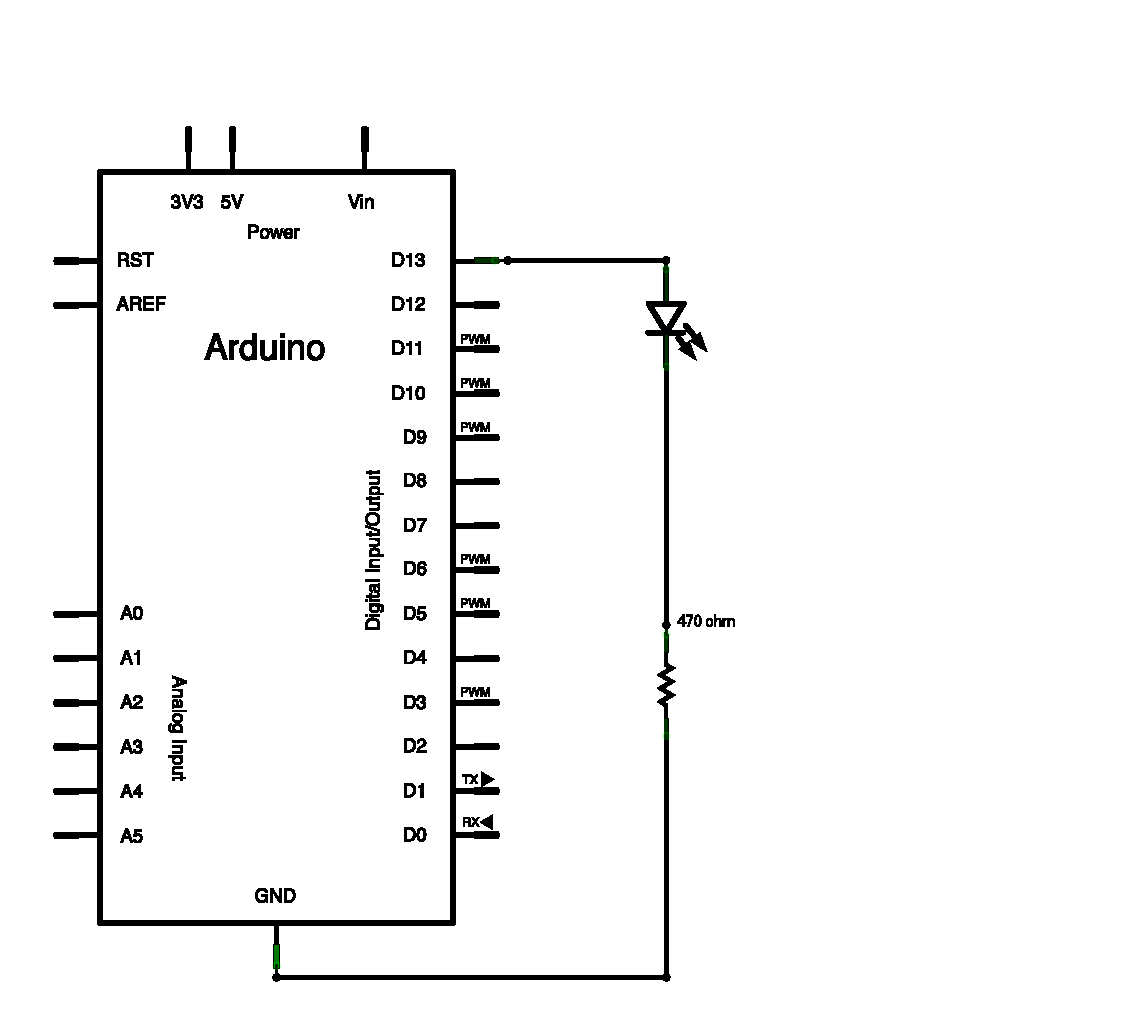
\includegraphics[width=0.9\linewidth]{images/ch2-one-led-circuit-schem}
		\captionsetup{labelformat=empty,justification=centering,font=footnotesize}
    \caption{A schematic of our circuit.}
    \label{diagram:ch2-one-led-circuit-schem}
  \end{center}
\end{wrapfigure}
%\end{figure}

Lastly, to complete the circuit, connect the negative side of the resistor to the {\code GND} pin on your Arduino with a jumper wire. You should now have a complete circuit that looks like Figure~\vref{diagram:ch2-one-led-circuit}. To the right is the equivalent circuit diagram that you might find in a text on electronics; you can see the source of the current (pin \chtwopin), the LED (the triangle with the arrows coming off of it), the resistor (a squiggly line),  and a connection back to ground (GND on the Arduino).


Now, you should be able to plug in the USB cable, and type in the code from this chapter. %If you compare the code in Listing~\vref{code:blink13} and the code in Listing~\vref{code:blink12}, you will see that we changed  one of the parameters to the procedure {\procname blink} on line 2. Instead of blinking pin {\constant 13}, we instead are asking the Arduino to blink pin {\constant 12}.

\newpage

\CODE

\lstinputlisting[caption=The {\procname blink} procedure lets you control how rapidly an LED blinks and which pin the LED is connected to.,label=code:blink13]{code/blink13.occ}

% I'm starting to wonder if this is ``Discussion'', or something.. 
\PATTERNS
In the previous chapter, we saw the {\procname heartbeat} procedure. In this chapter, we are introducing a new procedure called \blink. Unlike \heartbeat, \blink lets us control both which LED we are blinking as well as the speed at which the LED blinks.

On line 2, we can see that a \PROCedure called {\procname blink} is being called. This is just like {\procname heartbeat}---the code for that procedure is provided by the \plumbing environment. Note again the indentation---like \heartbeat (from Chapter~\ref{ch1}), \blink is indented by two spaces. However, instead of an empty set of parentheses (as was the case with \heartbeat), there is stuff in-between them. The numbers (\chtwopin and {\constant 500}) are the {\strong parameters} of the procedure \blink.

\begin{verbatim}
	blink (13, 500)
\end{verbatim}

{\strong Multiple parameters are always separated by a comma}.

Parameters are values that we give to procedures that let them do different things based on the values we provide. For example, the first parameter to the procedure {\procname blink} is the number {\constant 13}. This tells the Arduino which bit it should be turning on and off. Technically, we would say that the pin to which the LED is attached is being driven \HIGH and \LOW. As we explore more of the basics of electronics, you'll come to understand why we say \HIGH and \LOW instead of ``on'' and ``off.''


\begin{figure}[h!]
  \begin{center}
    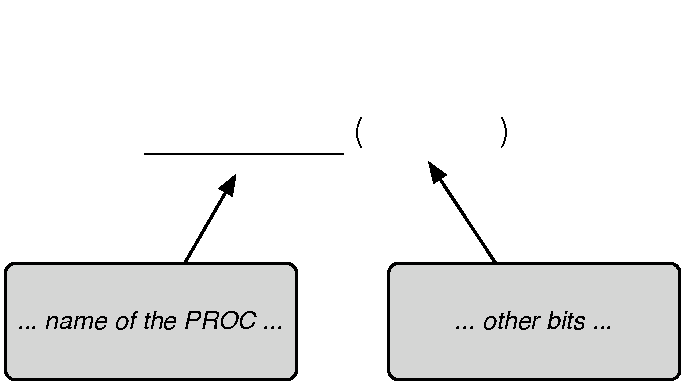
\includegraphics[width=\linewidth]{images/ch1-proc-call-pattern}
    \caption{Parameters go inside the parentheses.}
    \label{pattern:ch2-parameters}
  \end{center}
\end{figure}


The second parameter to \blink is the amount of time that we want to go by between when the LED is turned on and off. You might think that {\constant 500} is a rather large amount of time---until you realize that it is a value in {\em milliseconds}. The prefix {\em milli} means {\em one thousandth}. 1000 milliseconds (or 1000ms) equals 1 second. Therefore, half of a second is 500ms, and a tenth of a second is 100ms. 

\newpage

\section{Experimenting with Changes}
You can experiment with a few things at this point. For example, you could connect your LED up to pin {\constant 12} instead of \chtwopin. After changing the circuit, you would then need to modify your code.

\vspace{3mm}

\lstinputlisting[caption=Blinking an external LED on pin 12.,label=code:blink12]{code/blink12.occ}

The first parameter to \blink tells the procedure which pin it should be driving \HIGH and \LOW. If we connect the LED to pin 12 on the Arduino, we need to update the procedure call. Likewise, we can change the rate at which the LED blinks. Currently we are using the value {\constant 500}. What happens if you make it higher? Lower?

\BREAKAGE
There are a number of things that can break in this chapter.

\subsection{Break your circuit}
You've completed your first circuit. However, you might have done something wrong, in which case, nothing will work. You can intentionally break a few things without damaging your Arduino or burning out your LED.

\begin{description}
	\item[Flip the LED]\ \\ 
	If you flip the LED around, it won't light. In fact, it might burn out. Up to you if you want to test this.
	\item[Try another resistor]\ \\
	Try an 10k\ohm resistor instead of a 470\ohm resistor. You could try smaller resistors... but again, the LED might burn out. Up to you. (Trying larger values is safe.)
	\item[Wire wiggles]\ \\
	If you wiggle a wire out of place, you'll break the circuit. Then, nothing will work.
\end{description}

You can safely do each of these things, and see how your circuit fails to blink properly.

\subsection{Break your program}
There are quite a few ways you can break the software in this chapter---even though it is only three lines long!

\begin{description}
	\item[Wrong pin]\ \\
		If you forget to change the pin number from {\constant 13} to {\constant 12}, then you'll blink the wrong LED. Or, for that matter, if you blink pin {\constant 11}, nothing will appear to happen at all.
	\item[Crazy parameters]\ \\
	Try replacing the number {\constant 12} with {\code TWELVE}. See what happens. 
	
	\newpage
	
	\item[Crazy parameters II]\ \\
	Try replacing the number {\constant 12} with {\constant 122}. See what happens.
	\item[Too many parameters]\ \\
	Try using a parameter list like {\code 13, 12, 500}. That is, your code would look like:
	\begin{verbatim}
		blink (13, 12, 500)
	\end{verbatim}
	\item[Parameters too big]\ \\
	The parameter for the speed of the LED blink is an integer---a whole number without any decimal parts, if you prefer. Computers can only keep track of numbers that are so big (or small). How big can you make the blink speed? 
	\item[Blink too fast]\ \\
	What happens if you make the blink speed too small (e.g.~zero)?
	\item[Fractional blinking]\ \\
	What happens if you try and blink the LED every 100.5ms?
\end{description}

Remember, keeping track of the mistakes you make helps you know how to deal with them when you encounter them in your own programs later.


		



 


